\documentclass[aspectratio=43,11pt,hyperref={colorlinks=true}]{beamer}
\usetheme{boxes}
\setbeamertemplate{navigation symbols}{}
\definecolor{openstack}{RGB}{149,0,4}
\setbeamercolor{titlelike}{fg=openstack}
\setbeamercolor{structure}{fg=openstack}
\hypersetup{colorlinks,urlcolor=openstack}
\setbeamertemplate{footline}[frame number]
% Inserting graphics
\usepackage{graphicx}
% Side-by-side figures, etc
\usepackage{subfigure}
% Code snippits
\usepackage{listings}
% Color stuff
\usepackage{color}
\usepackage{amsmath}
\usepackage{tikz}
\newcommand\RBox[1]{%
  \tikz\node[draw,rounded corners,align=center,] {#1};%
}
\usepackage{hyperref}
%\usecolortheme{buzz}
%\usecolortheme{wolverine}
%\usetheme{Boadilla}
\usepackage[T1]{fontenc}

\definecolor{mygreen}{rgb}{0,0.6,0}
\definecolor{mygray}{rgb}{0.5,0.5,0.5}
\definecolor{mymauve}{rgb}{0.58,0,0.82}

\lstset{%
  backgroundcolor=\color{white},   % choose the background color; you must add \usepackage{color} or \usepackage{xcolor}
  breakatwhitespace=false,         % sets if automatic breaks should only happen at whitespace
  breaklines=true,                 % sets automatic line breaking
  captionpos=b,                    % sets the caption-position to bottom
  commentstyle=\color{openstack},  % comment style
  extendedchars=true,              % lets you use non-ASCII characters; for 8-bits encodings only, does not work with UTF-8
  keepspaces=true,                 % keeps spaces in text, useful for keeping indentation of code (possibly needs columns=flexible)
  keywordstyle=\color{blue},       % keyword style
%  otherkeywords={*,...},           % if you want to add more keywords to the set
  numbersep=5pt,                   % how far the line-numbers are from the code
  numberstyle=\tiny\color{mygray}, % the style that is used for the line-numbers
  rulecolor=\color{black},         % if not set, the frame-color may be changed on line-breaks within not-black text (e.g. comments (green here))
  showspaces=false,                % show spaces everywhere adding particular underscores; it overrides 'showstringspaces'
  showstringspaces=false,          % underline spaces within strings only
  showtabs=false,                  % show tabs within strings adding particular underscores
  stringstyle=\color{openstack},   % string literal style
}

\setbeamerfont{caption}{series=\normalfont,size=\fontsize{6}{8}}
\setbeamertemplate{caption}{\raggedright\insertcaption\par}

\setlength{\abovecaptionskip}{0pt}
\setlength{\floatsep}{0pt}

\author[Matthew Treinish]{%
    \texorpdfstring{%
        \centering
        Matthew Treinish\\
        \href{mailto:mtreinish@kortar.org}{mtreinish@kortar.org}\\
        \texttt{mtreinish on Freenode}
   }
   {Matthew Treinish}
}
\date{July 15, 2016}

\title[QA in the Open
\hspace{2em}\insertframenumber/\inserttotalframenumber]{QA in the Open}

\begin{document}

{%
\setbeamertemplate{background canvas}{
\includegraphics[width=\paperwidth,height=\paperheight]{background_title.png}}
\setbeamertemplate{footline}{}
\begin{frame}[noframenumbering]
    \setbeamercolor{titlelike}{fg=white}
    \setbeamercolor{structure}{fg=white}
    \setbeamercolor{normal text}{fg=white}
    \hypersetup{colorlinks,urlcolor=white}
    \setbeamercolor{author}{fg=white}
    \setbeamercolor{date}{fg=white}
    \setbeamercolor{background}{bg=openstack}
    \titlepage{}
    \centering
    \href{https://github.com/mtreinish/qa-in-the-open/tree/linuxcon-jp}{https://github.com/mtreinish/qa-in-the-open/tree/linuxcon-jp}
\end{frame}
}

\section{Open Source QA}
\begin{frame}
    \frametitle{What do I mean by Open Source QA}
    \begin{itemize}
        \item Doing Software QA in an Open Source manner
        \item Includes running tests and hosting results in the public
        \item Basically treat a project's QA like any other Open Source project
    \end{itemize}
\end{frame}

\begin{frame}
    \frametitle{My Personal Experiences with Enterprise QA}
    \begin{center}
        
\includegraphics[width=.85\textwidth]{facepalm.jpg}
    \end{center}
\end{frame}

\section{What is OpenStack QA?}
\begin{frame}
    \frametitle{What is OpenStack QA?}
    \begin{itemize}
     \item Official Mission Statement:\\
         \textit{Develop, maintain, and initiate tools and plans to ensure
the upstream stability and quality of OpenStack, and its release readiness at
any point during the release cycle.}
    \end{itemize}
\end{frame}

\begin{frame}
    \frametitle{Current QA Projects}
    \begin{columns}
        \column{.45\linewidth}
            \begin{itemize}
                \item{devstack}
                \item{devstack-plugin-cookiecutter}
                \item{devstack-plugin-ceph}
                \item{devstack-vagrant}
                \item{grenade}
                \item{tempest}
                \item{tempest-lib}
                \item{tempest-plugin-cookiecutter}
            \end{itemize}
        \column{.45\linewidth}
            \begin{itemize}
                \item{bashate}
                \item{stackviz}
                \item{hacking}
                \item{eslint-config-openstack}
                \item{os-testr}
                \item{os-performance-tools}
                \item{openstack-health dashboard}
                \item{karma-subunit-reporter}
            \end{itemize}
    \end{columns}
\end{frame}

\section{History of OpenStack QA}

\begin{frame}
    \frametitle{In The Beginning}
    \begin{itemize}
    \item Projects had unit tests
    \item Some projects had functional tests
    \item Testing was central to OpenStack culture
    \item But, no dedicated effort on QA or testing
    \end{itemize}
\end{frame}

\begin{frame}
    \frametitle{Then there was Tempest}
    \begin{itemize}
        \item The OpenStack integration suite
        \item Runs against a running OpenStack cloud via the REST APIs
        \item First dedicated QA effort in the community
    \end{itemize}
\end{frame}

\begin{frame}
    \frametitle{QA Becoming a Defined Group}
    \begin{itemize}
        \item 2 years later a separate project was created in governance around QA
        \item Started with just 2 projects: Tempest and Grenade
        \item Slowly started to consolidate several existing and add new projects
    \end{itemize}
\end{frame}

\begin{frame}
    \frametitle{Early Approach to QA}
    \begin{itemize}
        \item Only support for testing \textbf{Integrated} and
              \textbf{Incubated} projects
        \item Closer to a more traditional top down approach
        \item Testing was mostly unit tests and tempest tests
        \item All integrated and incubated projects had to co-gate against
              each other in 1 large integrated gate queue
    \end{itemize}
\end{frame}

\begin{frame}
    \frametitle{OpenStack Project Growth}
    \begin{center}
        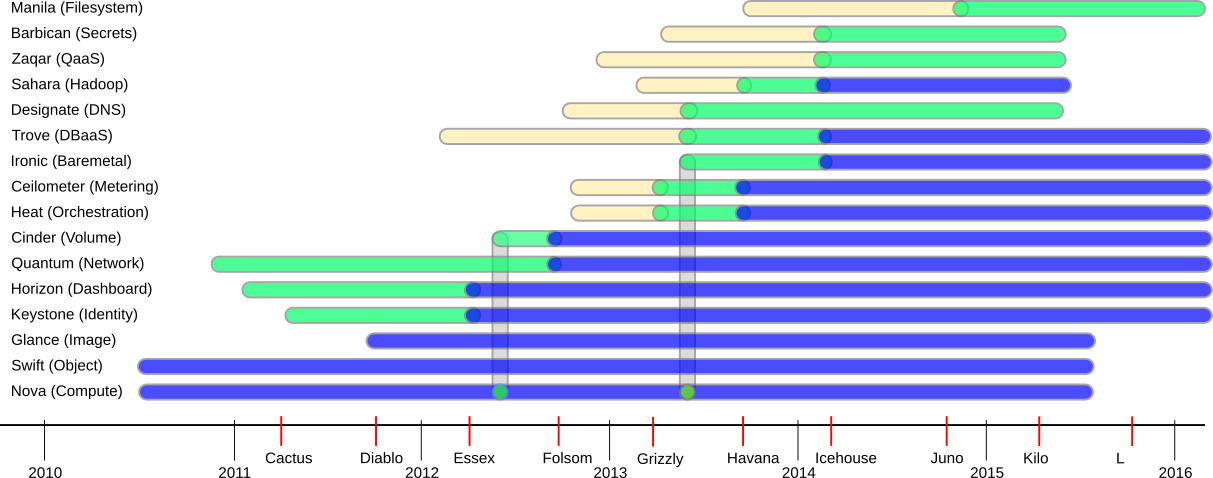
\includegraphics[width=1.1\textwidth]{OpenStack_Components.png}
    \end{center}
\end{frame}

\begin{frame}
    \frametitle{QA Growing Pains}
    \begin{itemize}
        \item QA Projects have a small core review team
        \item Limited expertise on newer projects
        \item Project teams weren't motivated to contribute
    \end{itemize}
\end{frame}

\begin{frame}
    \frametitle{Tempest Tests per Project}
    \begin{center}
        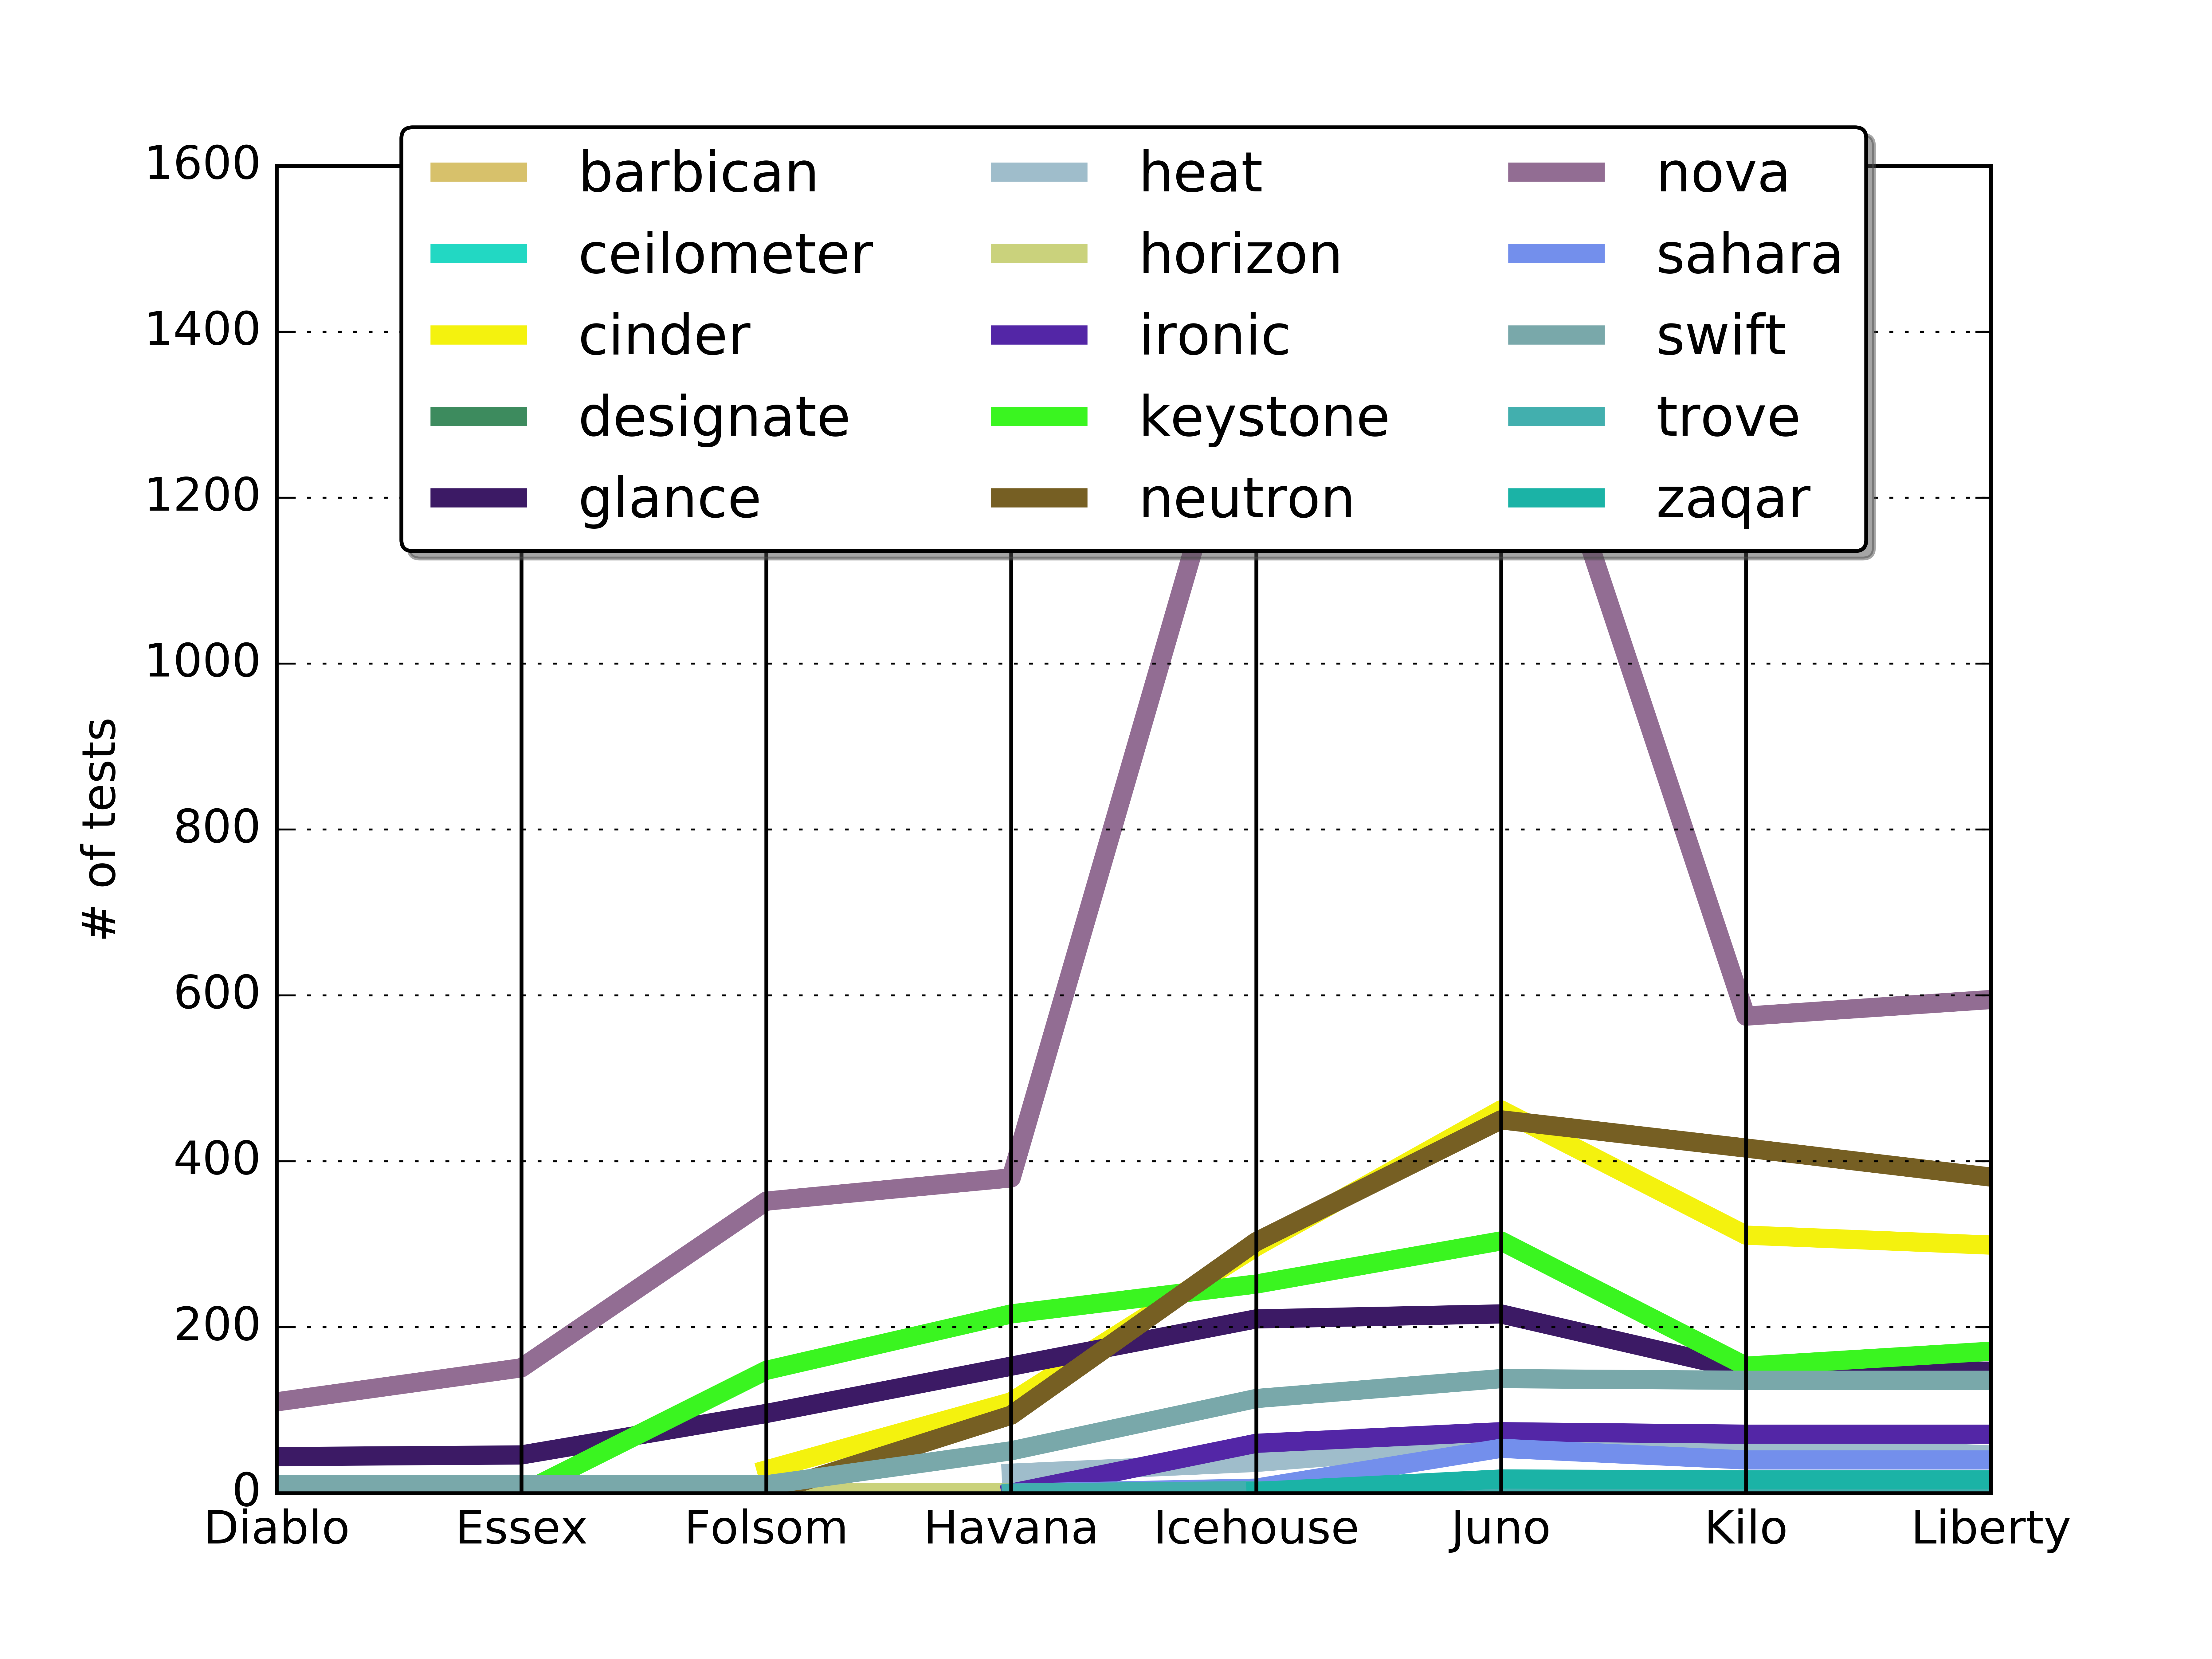
\includegraphics[width=.95\textwidth]{tests_per_proj.png}
    \end{center}
\end{frame}

\begin{frame}
    \frametitle{The Big Tent}
    \begin{itemize}
        \item OpenStack's most recent governance change
        \item Went from having a strict 2 stage approval process and a small
            set of OpenStack projects to a more inclusive approach
        \item Integrated and incubated projects no longer a thing
        \item Designed to switch from choosing winners to building an ecosystem
    \end{itemize}
\end{frame}

\begin{frame}
    \frametitle{The Big Tent\ldots}
    \begin{center}
        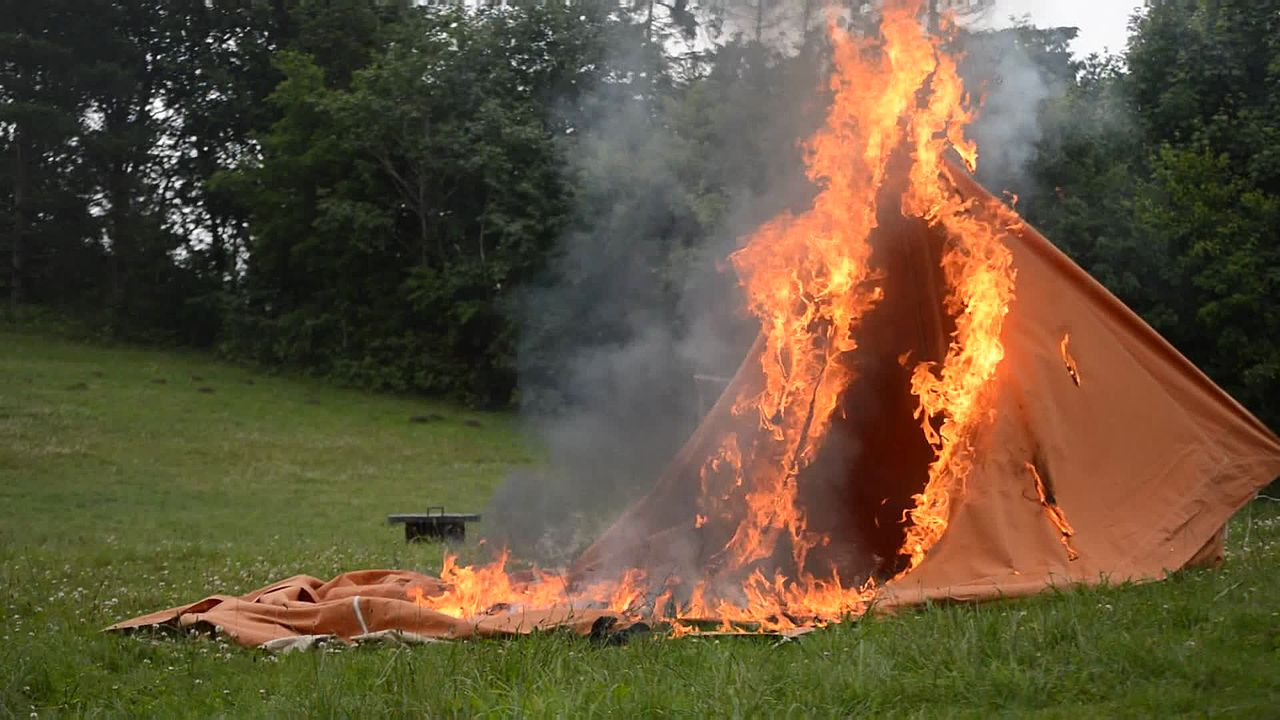
\includegraphics[width=.9\textwidth]{Burning_Tent.jpg}
    \end{center}
\end{frame}

\begin{frame}
    \frametitle{QA in the Big Tent}
    \begin{itemize}
        \item QA projects will still provide direct support for base IaaS projects
        \item Provide stable plugin interfaces to expand functionality for other projects
        \item Better fits with the growth in projects
    \end{itemize}
\end{frame}

\begin{frame}
    \frametitle{Introducing Plugin Interfaces}
    \begin{itemize}
        \item Add stable interfaces to expand QA project functionality
        \item Enable any project to self service their own QA
        \item Concentrate on making things in QA projects externally reusable
        \item Started with Devstack, now Tempest and Grenade too
    \end{itemize}
\end{frame}

\section{Conclusions}

\begin{frame}
    \frametitle{Lessons from OpenStack QA}
    \begin{center}
        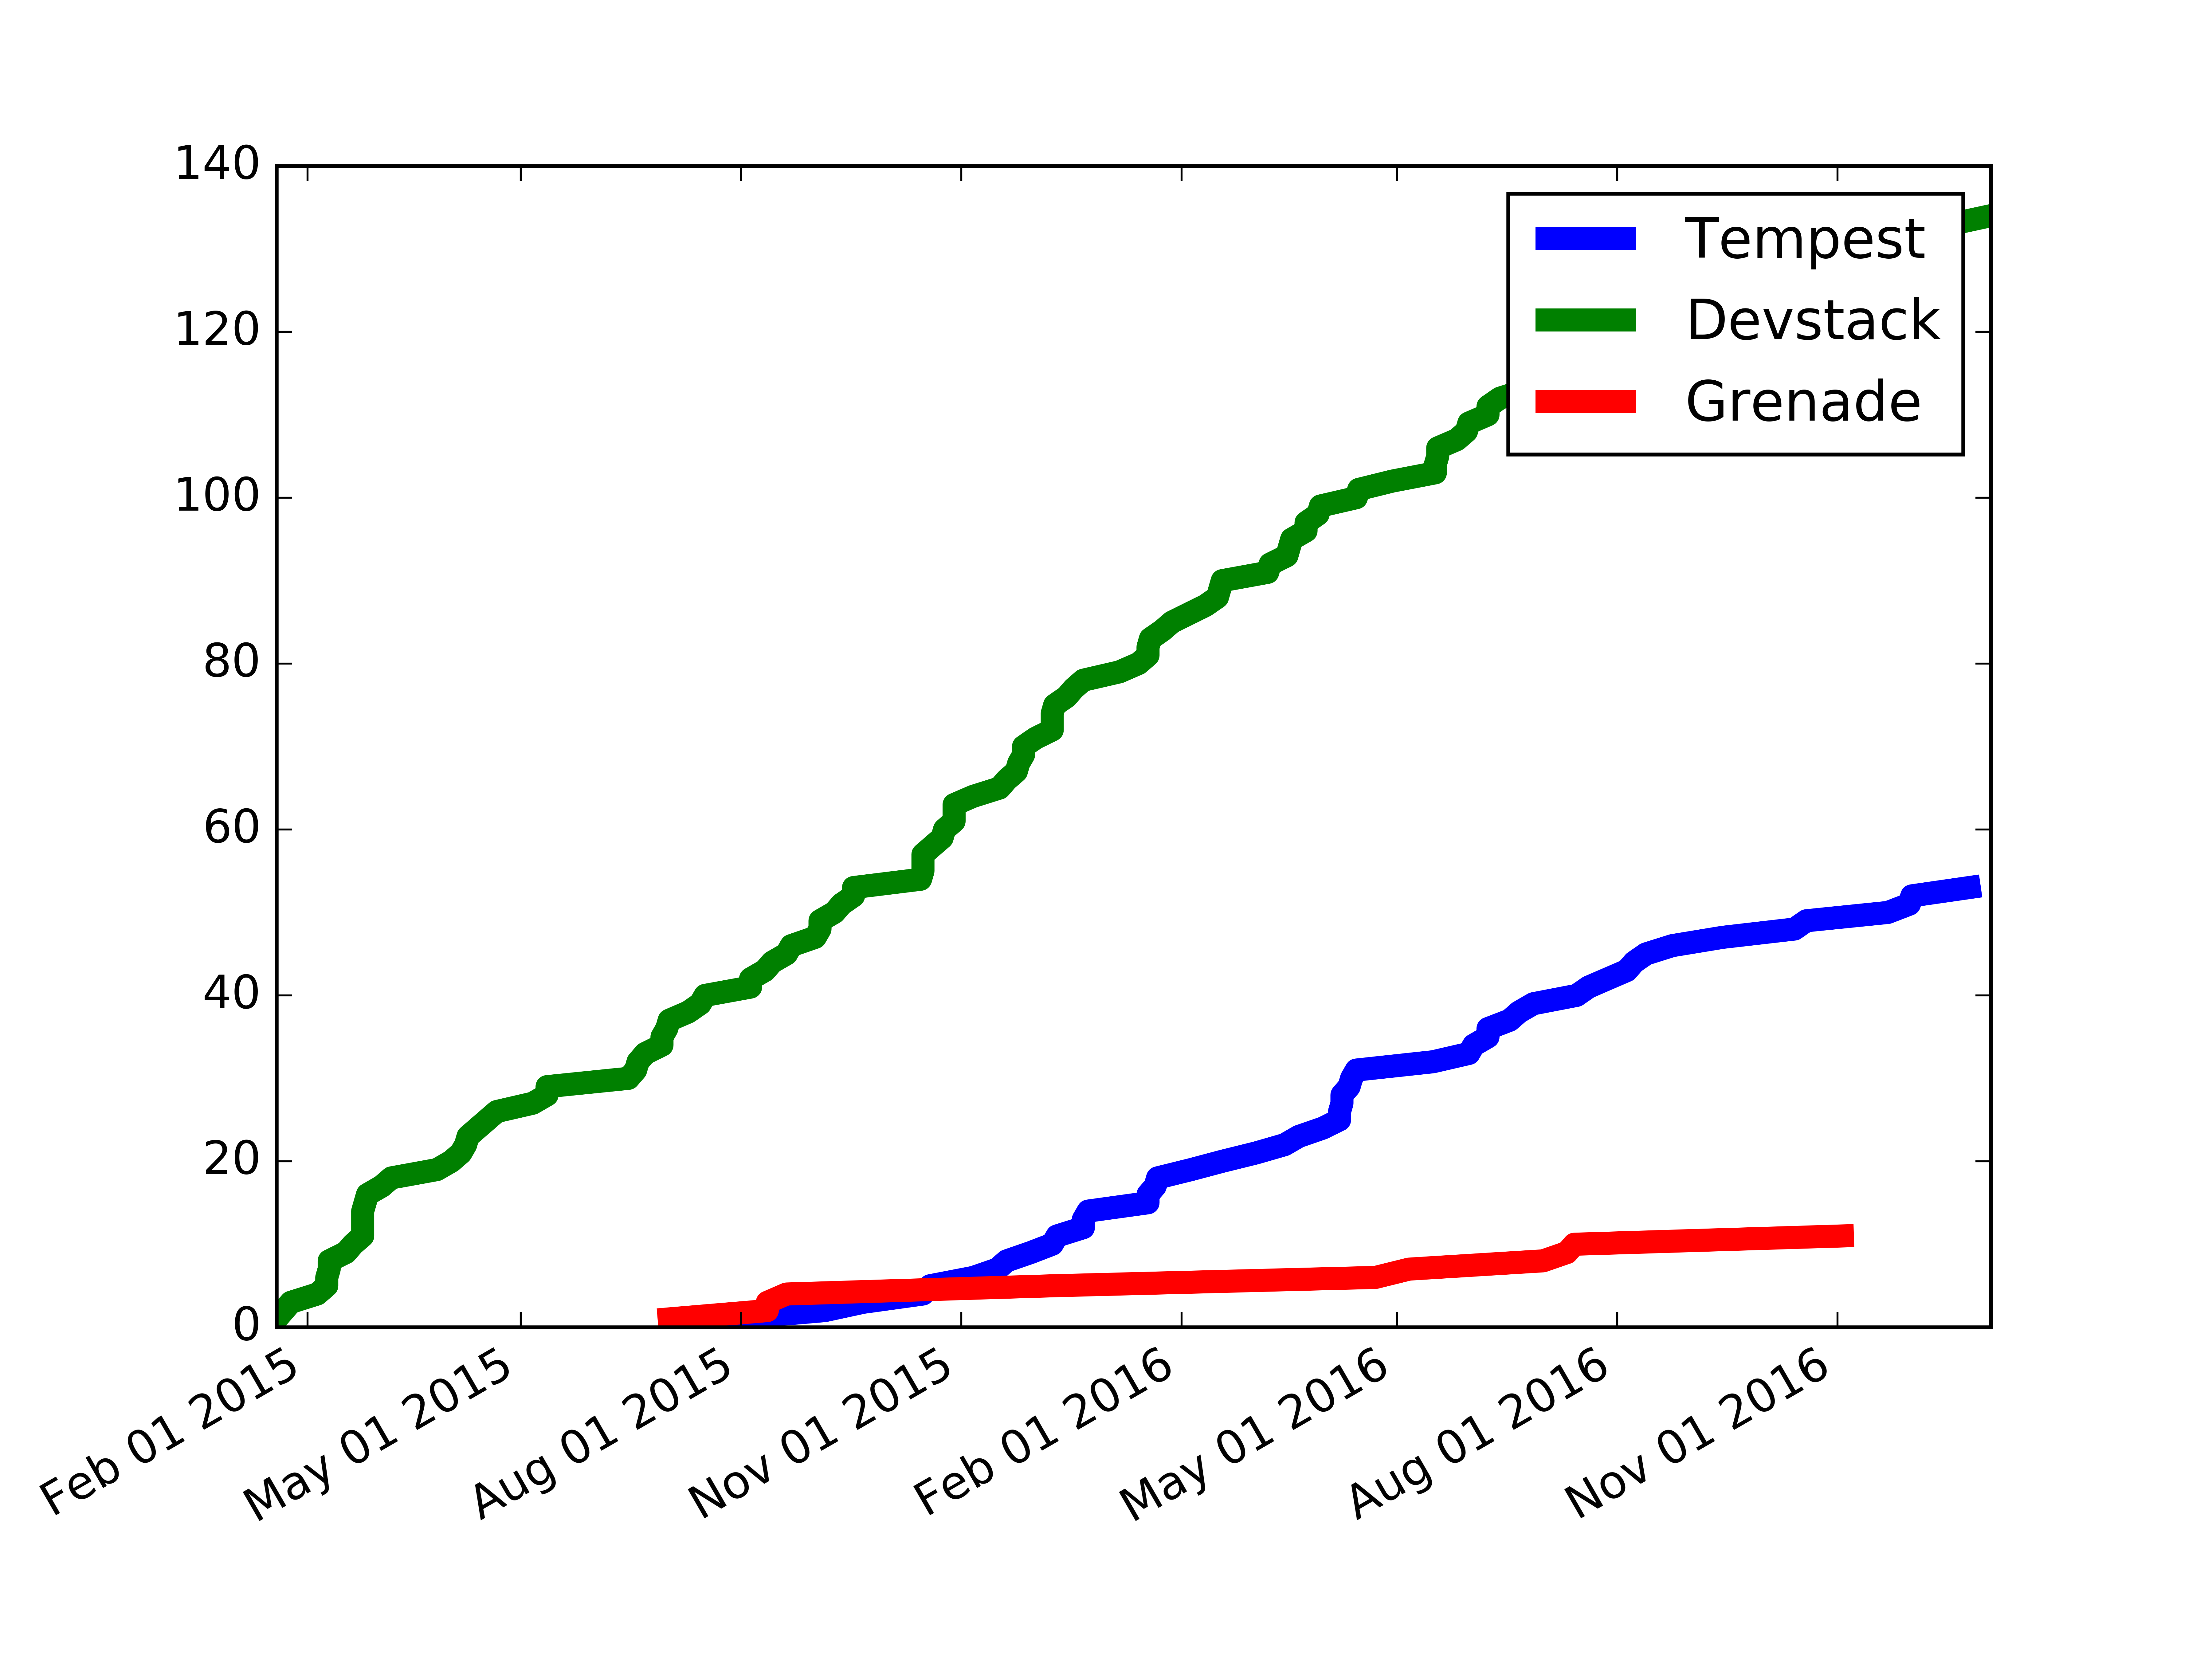
\includegraphics[width=.6\textwidth]{plugins.png}
    \end{center}
    \begin{itemize}
        \item Monolithic and Separate doesn't scale
        \item Keeping Things Separate increases friction
    \end{itemize}
\end{frame}

\begin{frame}
    \frametitle{Advantages}
    \begin{itemize}
        \item Enables external audit of testing
        \item User confidence in project
        \item Enables indpendently repeatable testing
        \item Reusable components
    \end{itemize}
\end{frame}

\begin{frame}
    \frametitle{Potential Issues}
    \begin{itemize}
        \item Lack of Corporate Contribution
        \item Limited Free Resources for running tests
        \item Sometimes difficult to get community buy in
    \end{itemize}
\end{frame}

\section{More Information}
\begin{frame}
\frametitle{Where to get more information}
    \begin{itemize}
        \item openstack-dev ML\: \href{mailto:openstack-dev@lists.openstack.org}{openstack-dev@lists.openstack.org}
        \item \#openstack-qa on Freenode
        \item \href{https://wiki.openstack.org/wiki/QA}{https://wiki.openstack.org/wiki/QA}
    \end{itemize}
\end{frame}

\section{Questions}
\begin{frame}
\frametitle{Questions?}
\end{frame}

\end{document}
